% !TeX spellcheck = cs_CZ
\wikitextrule
\begin{example}\label{MAI:exam031}
  Je dána funkce \(f: f(x) = \frac{x + 1}{x}\). Sledujme její chování, když hodnoty argumentu \(x\) 
  budou vzrůstat 
  nade všechny meze neboli, jak říkáme, \(x\) se bude blížit k \(+\infty\) (což zapisujeme \(x \to 
  + \infty\) (viz obr. \ref{mai_fig019}). Můžeme psát \(f(x) = 1 + 1/x\). Vzrůstají-li neomezeně 
  hodnoty proměnné \(x\), blíží se hodnoty výrazu \(1/x\) čím dál tím více nule, takže funkční 
  hodnoty \(f(x)\) jsou čím dál tím blíže číslu \(1\). V tomto případě píšeme \(lim_{x\to+\infty} 
  f(x) = 1\) nebo \(f(x) \to 1\) pro \(x\to +\infty\) a říkáme, že funkce \(f\) má v bodě 
  \(+\infty\) limitu rovnou \(1\). Přesně to znamená toto: Zvolíme-li libovolně malé \(\varepsilon 
  > 0\), můžeme nalézt \(p > 0\) tak, že pro \(x > p\) platí \(\abs{f(x) — l} < \varepsilon\). (Viz 
  obr. \ref{mai_fig019}.) Můžeme to říci i takto: Zvolíme-li libovolně okolí bodu \(1\), existuje 
  okolí bodu \(+\infty\) tak, že pro každé \(x\) (konečné) z tohoto okolí je \(f(x)\) ve zvoleném 
  okolí bodu \(1\).
  
  {\centering
   \captionsetup{type=figure}
%   % !TeX spellcheck = cs_CZ
% xelatex -enable-write18 -shell-escape mai_fig020.tex
\documentclass[11pt]{standalone}
\usepackage{xltxtra}
\usepackage[usenames,x11names]{xcolor}
\usepackage{tikz}
  \usetikzlibrary{intersections}
  \usetikzlibrary{decorations.markings}
\usepackage{pgfplots}
  \pgfplotsset{compat=newest}
  
\usepackage{amsmath}

\begin{document}
  \begin{tikzpicture}[thick,scale=0.7, 
      every node/.style={transform shape},
      ]
  
  \tikzset{->-/.style={decoration={
    markings,
    mark=at position #1 with {\arrow{stealth}}},postaction={decorate}}}
    
    \begin{axis}[
      xmin = -2, xmax = 3.5, ymin = -2, ymax = 6,  % osy
      domain =-2:8,
      restrict y to domain=-1.5:6,
      axis equal image,
      grid = major,   % both
      grid style={line width=.1pt, draw=gray!20},
      major grid style={dashed, line width=.2pt, draw=gray!40},
      clip = true,
      clip mode=individual,
      xtick={-1,0,1,2,3,4}, % make steps of length 0.2
      ytick={-1,0,1,2,3,4,5,6,7,8}, 
      axis x line = middle,
      axis y line = middle,
      xlabel={$x$}, ylabel={$y$},
      enlarge y limits={rel=0.07},
      enlarge x limits={rel=0.07},
      ]
  
      \addplot[color=Gold3, samples=100, smooth, ultra thick, unbounded coords=jump,
               no markers, domain = -2:2, name path global=func1] 
         gnuplot{x^3};
  
      \node [fill=white] at (rel axis cs: 0.85,0.9) {\(y=x^3\)};
  
      \path[name path=line] (1.5,0) -- (1.5,6); 
          % Intersections points
          \path [name intersections={of=func1 and line,by={P1}}] (P1) node [] {};
          \draw[->-=.4, dashed, gray] (P1 |- 3,-0.05) node[below, fill=white] {\(x\)} -- (P1);
          \draw[->-=1,  dashed, gray] (P1) -- (P1 -| 0,3) 
            node[left=0.5cm, fill=white] {\small\(f(x)\)};
          \draw[dashed, gray] (P1 -| 0,3) + (-0.6cm,0cm) -- (P1 -| 0,3);
      \path[name path=line1] (0,1) -- (2,1); 
          % Intersections points
          \path [name intersections={of=func1 and line1, by={P1}}] (P1) node [] {};    
          \path (P1 |- 3,-0.1) node [below, fill=white] (X) {p} -- (P1) -- (P1 -| 0,3) 
              node[left, fill=white] (Y) {\(q\)};
  
      \draw[thick,red, fill=white] ([shift=(90:2mm)]X) 
           arc (270:360:1mm) node(x1) {} arc (360:450:1mm);
      \draw[dashed] (P1 |- 3,-0.1) -- (P1) -- (P1 -| 0,3);
      \draw[line width = 1pt,red] (x1 |- 3,0)  -- (3,0);
      
      \draw[thick,red] (0,1) -- (0,6);
      \draw[thick,red, fill=white] ([shift=(0:3.3mm)]Y) arc (0:180:1mm);;
    \end{axis}
  \end{tikzpicture}
\end{document}
   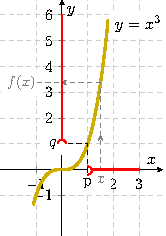
\includegraphics[width=0.45\linewidth]{mai_fig020.pdf}
   \captionof{figure}{K příkladu \ref{MAI:exam031}
   \cite[s.~119]{Brabec1989}
   \label{mai_fig020}}
  \par}
\end{example}















